%% 
%% Copyright 2019 Elsevier Ltd
%% 
%%
%%%%%%%%%%%%%%%%%%%%%%%%%%%% ! ! ! SUBMISSION CHECKLIST ! ! ! %%%%%%%%%%%%%%%%%%%%%%%%%%%%
%%
%% Please confirm that your submission follows all the requirements of the guidelines, including the submission checklist:
%% _ Cover letter
%% _ Highlights
%% _ Authorship statement
%% _ The manuscript must be single column and double spaced
%% _ Reference must be in the author-date format
%% _ Code availability section 
%%
%% *All the manuscripts in disagreement with the guidelines will be desk-rejected without editorial check.
%%
%% --------------------------------------
%%
%% This file is part of the 'CAS Bundle'.
%%  
%% It may be distributed under the conditions of the LaTeX Project Public
%% License, either version 1.2 of this license or (at your option) any
%% later version.  The latest version of this license is in 
%%    http://www.latex-project.org/lppl.txt 
%% and version 1.2 or later is part of all distributions of LaTeX
%% version 1999/12/01 or later.
%%   
%% The list of all files belonging to the 'CAS Bundle' is
%% given in the file `manifest.txt'.
%% 
%% Template article for cas-dc documentclass for  
%% double column output.
 
%\documentclass[a4paper,fleqn,longmktitle]{cas-dc}
\documentclass[a4paper,fleqn]{cas-sc}

\usepackage[authoryear]{natbib}
\usepackage{graphicx} 
\usepackage{float}
\usepackage{algorithm}  
\usepackage{algpseudocode}
\usepackage{color}
\usepackage{setspace}
\usepackage[nomarkers,figuresonly]{endfloat}


\newcommand{\colorComments}{black} 
 
%%%Author definitions
\def\tsc#1{\csdef{#1}{\textsc{\lowercase{#1}}\xspace}}
\tsc{WGM}
\tsc{QE}
\tsc{EP}
\tsc{PMS}
\tsc{BEC}
\tsc{DE}
%%%

\usepackage{lineno}
\linenumbers 

\begin{document}
\let\WriteBookmarks\relax
\def\floatpagepagefraction{1}
\def\textpagefraction{.001}
\shorttitle{Combining class-weighted algorithm and machine learning models in landslide susceptibility mapping}
\shortauthors{Huijuan Zhang and Yingxu Song et al}

\title [mode = title]{Combining class-weighted algorithm and machine learning models in landslide susceptibility mapping: a case study of Wanzhou section of the Three Gorges Reservoir, China}

\author[1,2]{Huijuan Zhang}[]
\credit{Conceptualization, Validation, Writing-original draft preparation, Writing-review and editing}

\author[3]{Yingxu Song} [type=editor,
auid=000,bioid=1,orcid=0000-0002-9273-2019]
\credit{Conceptualization, Methodology, Software, Validation, Investigation, Resources, Funding acquisition}

\author[4]{Shiluo Xu}
\credit{Software, Resources}

\author[5]{Yueshun He}
\credit{Project administration, Funding acquisition}

\author[6]{Zhiwen Li}
\credit{Conceptualization}

\author[7]{Xianyu Yu}
\credit{Resources, Funding acquisition}

\author[8]{Ye Liang}
\credit{Funding acquisition}

\author[1]{Weicheng Wu}
\credit{Writing-review and editing}

\author[2]{Yue Wang}
\credit{Software}

\address[1]{Key Lab of Digital Land and Resources and Faculty of Earth Sciences, East China University of Technology, Nanchang, 330013, Jiangxi, China}
\address[2]{School of Earth Sciences, East China University of Technology, Nanchang, Jiangxi Province 330013, China}
\address[3]{Jiangxi Engineering Laboratory on Radioactive Geoscience and Big Data Technology, School of Information and Engineering, East China University of Technology, Nanchang, 330013, Jiangxi, China; yxsong@ecut.edu.cn}
\address[4]{School of Information Engineering, Huzhou University, Huzhou 313000, China; xushiluo@163.com} 
\address[5]{East China University of Technology, Nanchang, 330013, Jiangxi, China; heys@ecut.edu.cn} 
\address[6]{School of Environmental and Chemical Engineering, Foshan University, Foshan, 528000, China; lizw1982@163.com} 
\address[7]{School of Civil Engineering, Architecture and Environment, Hubei University of Technology, Wuhan, Hubei Province 430074, China; yuxianyu@hbut.edu.cn} 
\address[8]{Jiangxi Engineering Technology Research Center of Nuclear Geoscience Data Science and System, East China University of Technology, Nanchang, 330013, Jiangxi, China; liangye@ecut.edu.cn} 
\address[1]{Key Lab of Digital Land and Resources and Faculty of Earth Sciences, East China University of Technology, Nanchang, 330013, Jiangxi, China; wuwch@ecut.edu.cn/wuwc030903@sina.com} 
\address[2]{School of Earth Sciences, East China University of Technology, Nanchang, Jiangxi Province 330013, China; 2020210058@ecut.edu.cn} 


\begin{abstract}
This study aims to investigate the application of the class-weighted algorithm combined with traditional machine learning (logistic regression) and ensemble machine learning models (LightGBM and random forest) to the landslide susceptibility evaluation. 
Wanzhou section of the Three Gorges Reservoir area, China, which have numerous landslides and the number of landslide samples is 19 times more than non-landslide samples, is chosen as an example. 
The class-weighted algorithm focuses on the class-imbalanced problem of landslide and non-landslide samples in the assessment of landslide susceptibility and can turn the class-imbalanced issue into a cost-sensitive problem by setting unequal weights for different classes, which contribute to improving landslide susceptibility evaluation accuracy.   
The landslide inventory database was produced by field investigation and remote sensing images derived from Google Earth. 
Of the 233 landslides in the inventory, 40\% were used for validation, and the remaining 60\% were used for training purposes. 
Twelve environmental parameters (elevation, slope, aspect, curvature, distance to river, NDVI, NDWI, rainfall, seismic intensity, land use, TRI, lithology) were treated as inputs of the models to produce landslide susceptibility map (LSM). The AUC value, Balanced accuracy, and Geometric mean score were utilized to estimate the quality of models. 
The results showed that the weighted models (weighted logistic regression, weighted LightGBM, weighted random forest) have higher AUC values, Balanced accuracy, and Geometric mean scores than those of unweighted methods, which demonstrated that the weighted models exhibit better than unweighted methods, with the weighted random forest method having the best performance. 
The landslide susceptibility map of the Wanzhou section display that the high and very high landslide susceptibility are mainly distributed on both sides of the river. 
The insights from this research will be useful for ameliorating the landslide susceptibility mapping and the development of prevention and mitigation Wanzhou section. 
\end{abstract}
 
\begin{coverletter}

Dear Editors-in-Chief,
\newline

please find the enclosed manuscript "Combining class-weighted algorithm and machine learning models in landslide susceptibility mapping: a case study of Wanzhou section of the Three Gorges Reservoir, China" which we are submitting for exclusive consideration for publication in Computers \& Geosciences. We confirm that the submission follows all the requirements and includes all the items of the submission checklist.  
\newline

In this contribution, to solve the imbalanced landslide samples (landslides, non-landslides) in the landslide susceptibility evaluation, the application of the class-weighted algorithm combined with traditional machine learning (logistic regression) and ensemble machine learning models (LightGBM and random forest) have been investigated. 
Wanzhou section of the Three Gorges Reservoir area, China, where the number of landslide samples is 19 times more than non-landslide samples, is chosen as an example. 
The landslide inventory database was produced using field investigation and remote sensing images provided by Google Earth. Of the 233 landslides in the inventory, 40\% were used for validation, and the remaining 60\% were used for training purposes. Twelve environmental parameters (elevation, slope, aspect, curvature, distance to river, NDVI, NDWI, rainfall, seismic intensity, land use, TRI, lithology) were used as inputs of the models to produce landslide susceptibility map (LSM). 
The AUC value, Balanced accuracy, and Geometric mean score were used to estimate the quality of models. 
Research has found that the weighted models (weighted logistic regression, weighted LightGBM, weighted random forest) are better than unweighted methods and the weighted random forest method has the best performance. 
The class-weighted algorithm turned the susceptibility evaluation problem into a cost-sensitive problem by setting unequal weights for different classes, which is probably to be applied to the landslide susceptibility evaluation in other areas.
\newline

We provide the source codes in a public repository with details listed in the section "Code availability".
\newline

Thanks for your consideration. 
\newline
Sincerely,
\newline

Yingxu Song
\newline
Jiangxi Engineering Laboratory on Radioactive Geoscience and Big Data Technology, School of Information and Engineering, East China University of Technology, Nanchang, 330013, Jiangxi, China; yxsong@ecut.edu.cn
\end{coverletter}

 
\begin{highlights}
\item The imbalanced landslide samples (landslides, non-landslides) in the landslide susceptibility evaluation is emphasized.
\item The class-weighted algorithm combined with machine learning (Logistic regression) and ensemble machine learning models (LightGBM and random forest) were applied to the landslide susceptibility evaluation.
\item The weighted models are applicable for solving the problem of imbalanced landslide samples and have improved the landslide susceptibility mapping well.
\end{highlights}

\begin{keywords}
landslide susceptibility mapping\sep class-weighted algorithm \sep imbalanced landslide data \sep machine learning model \sep Three Gorges Reservoir area
\end{keywords}

\maketitle 

\printcredits

\doublespacing


\section{Introduction}

Landslide refers to a natural phenomenon in which the soil or rock mass on the slope slides downwards along the soft surface under the action of gravity or other external forces.
Landslide is a common geological disaster, causing many economic losses and unfor-tunate casualties, such as devastating soil, vegetation, and dwellings, as well as critically blocking transportation lines and waterways\citep{Abuzied2016JoMS, 2017Chenp147160}.
The China Geological Survey reported that there were 6181 geological disasters in 2019, including landslides, collapses, mudrock flows, the ground collapses, ground fissures, and land subsidence, resulting in 211 deaths, 13 missings, 75 injured and direct economic losses of 2.77 billion Yuan.
Among them, 4020 landslides occurred, mainly distributed in Southwestern China, and brought about a large number of missing persons and severe economic losses.
Various factors, such as natural factors (e.g., heavy rainfall, earthquake, loose lithology, and low vegetation coverage, etc.) and human-made factors (e.g., infrastructures con-struction and road irrigation, etc.) can trigger landslides\citep{2018Wildep97104}.
Especially in recent years, the rapid urbanization and industrialization have increased the likelihood of landslide occurrence \citep{2020Kocamanp118}, which led to higher number of human casualties and more enormous loss of property. 
It is therefore of significant necessity to develop landslide susceptibility map, which represents the probability of the spatial distribution of landslides in a specific region based on historical landslides and related factors \citep{2016Yup487487,Song2018}.Government agencies have attempted to take various measures to reduce the casualties and financial losses caused by landslides. 
This process generally involves carrying out LSM, representing the probability of the spatial distribution of landslides in a specific region based on historical landslides and related factors \citep{2016Yup487487,Song2018}. 
Landslide susceptibility map can help government agencies to take preventable measures for reducing the casualties and financial losses caused by landslides.

Various methods and techniques, which can be defined as qualitative or quantitative, have been implemented in the landslide susceptibility assessment and have achieved notable progress \citep{Fang2020IJoGIS,Guzzetti_1999_Geomorphology,Bui2020Catena}. 
Qualitative methods are based on expert knowledge to identify the main triggering factors, determine the weights of natural and human-made factors and acquire landslide susceptible zones \citep{Aditian2018Geomorphology}, such as analytic hierarchy process (AHP) (Barredo et al., 2000; Yalcin, 2008; Feizizadeh et al., 2014)\citep{Barredo2000IJoAEOaG,Yalcin2008Catena}, interval pairwise comparison matrix (IPCM)\citep{Ghorbanzadeh2019RemoteSensing}, and fuzzy logic models\citep{Aksoy2012Computers&Geosciences,Anbalagan2015GeoenvironmentalDisasters,Shahabi2015EnvironmentalEarthSciences,Roy2019RemoteSensingApplicationsSocietyandEnvironment}. 
Whereas quantitative methods rely on mathematical models including the statistical and deterministic models\citep{Abuzied2016JoMS, Reichenbach2018ER,Fang2020IJoGIS}. 
With the rapid advancement of computer technology and the improvement of remote sensing (RS) and geographic information system (GIS) technology, the quantitative methods develop swiftly. 
Many studies have demonstrated that the quantitative approaches are more precise than qualitative methods because the qualitative methods have much subjectivity concerning the prediction of landslides\citep{Aditian2018Geomorphology, Bui2020Catena}. 
Machine learning model which is one of the qualitative methods has the capability of handling non-linear data with different scales and from different type of sources\citep{Bui2020Catena}. 
Different machine learning algorithms together with GIS and RS techniques have been widely applied to assess landslide susceptibility and perform well, such as LR (logistic regression), which were most widely used and often found successful in the landslide susceptibility evaluation (wenxian12/13) (Ayalew and Yamagishi, 2005; Eeckhaut et al., 2006; Bai et al., 2010; Akgun, 2012)\citep{2019Sevgenp39403940}. 
Additionally, the ensemble learning methods acting as an improvement of traditional machine learning models arise and show more robust performance in many real-world tasks, widely used in landslide susceptibility evaluation (Althuwaynee et al., 2014; Napoli et al., 2020; Hong et al., 2020; Saha et al., 2021). 
Random forest (RF) (Breiman, 2001), which is an extended variant of the bagging method, has a simple implementation and low computational overhead (Youssef et al., 2015; Kim et al., 2017). LigthGBM is a new member of the boosting ensemble models, having faster training efficiency, higher accuracy, and more robust ability to handle large-scale data (Song et al., 2018). 
However, landslide samples are often much less than non-landslide samples in almost every study region, leading to poor performance in landslide susceptibility evaluation whether the traditional machine learning or ensemble machine learning models are utilized.
Some researchers have paid attention to the sample selection in the evaluation of landslide susceptibility, \citep{Ada2017NH,San2014IJoAEOaG,Nefeslioglu2012IJoAEOaG}.


The class-weighted algorithm treats the susceptibility assessment as a cost-sensitive issue and sets different misclassification weights for different categories (landslides, non-landslides). 
This method has been widely used to solve the unbalanced variety, but the application to landslide susceptibility assessment is still relatively few. 

Wanzhou district of Chongqing is in the Three Gorges Reservoir area's hinterland, playing a significant role in the prevention and domination of geological disasters in the Three Gorges Reservoir area. In recent decades, because of the abundant precipitation and cyclical fluctuation of water level in the Yangtze River, landslides and other geological disasters in this area have increased significantly, seriously destroying the eco-logical environment and socially sustainable development. 
In this study, the Wanzhou section of Three Gorges Reservoir was selected as the research area, and the class-weighted algorithm combined with traditional machine learning model (Logistic regression) and ensemble machine learning models (LightGBM and random forest) were applied to the landslide susceptibility evaluation. 
The purpose of this research attempts to achieve the relatively optimal method in which the impact of unbalanced landslide samples can be minimized, and the accuracy of the landslide susceptibility map is improved, providing essential introductory information for mitigating the land-slide hazard by governmental subdivisions or decision-makers. 
Different from previous work, the novelty of this paper are 1) the class-weighted algorithm is firstly applied to landslide susceptibility mapping; 2) the advantages and disadvantages of traditional machine learning model (Logistic regression) and ensemble machine learning models (LightGBM and random forest) combined with class-weighted algorithm were com-pared in the Wanzhou section.


\label{intro}



Examples of citations:

\cite{gomez1990isim3d, pebesma2004multivariable, hansen2018multiple}

Examples of citations in parentheses: 

\citep{gomez1990isim3d, pebesma2004multivariable, hansen2018multiple}

\section{Methodology}

This section includes an example of equation. 
 
\begin{equation}
\label{eqn:linear}
    y=ax+b.
\end{equation}


\subsection{Subsection}

This section contains another example of equation, different from Eq.  \ref{eqn:linear}.

\begin{equation} 
\label{eqn:quadratic}
    y=ax^2+bx+c
\end{equation}

\section{Algorithm and implementation}

Example of algorithm:
\begin{algorithm}
  \caption{Algorithm example }
  
  \begin{algorithmic}
  \label{alg:Alg1}
  \State \textbf{Input:} ...
   \newline

 \Statex \textit{1.} Step1
  \Statex \textit{2.} Step2;
 \State \textit{3.}  Step3;
  \newline
   \For{ i = 1,..., m}
   \State \textit{4.} Step 4;
    \For{ j = 2,..., n} 
   \State \textit{5.}  Step 5;
   \State \textit{6.} Step 6;
   \EndFor
  \EndFor 
  \newline
\State  \textbf{Output: } ... 
  \end{algorithmic} 
\end{algorithm} 


\section{Results}


This section includes an example of figure (Figure \ref{fig:Figure1}), from  \cite{de2021direct}.

\begin{figure}
\centering
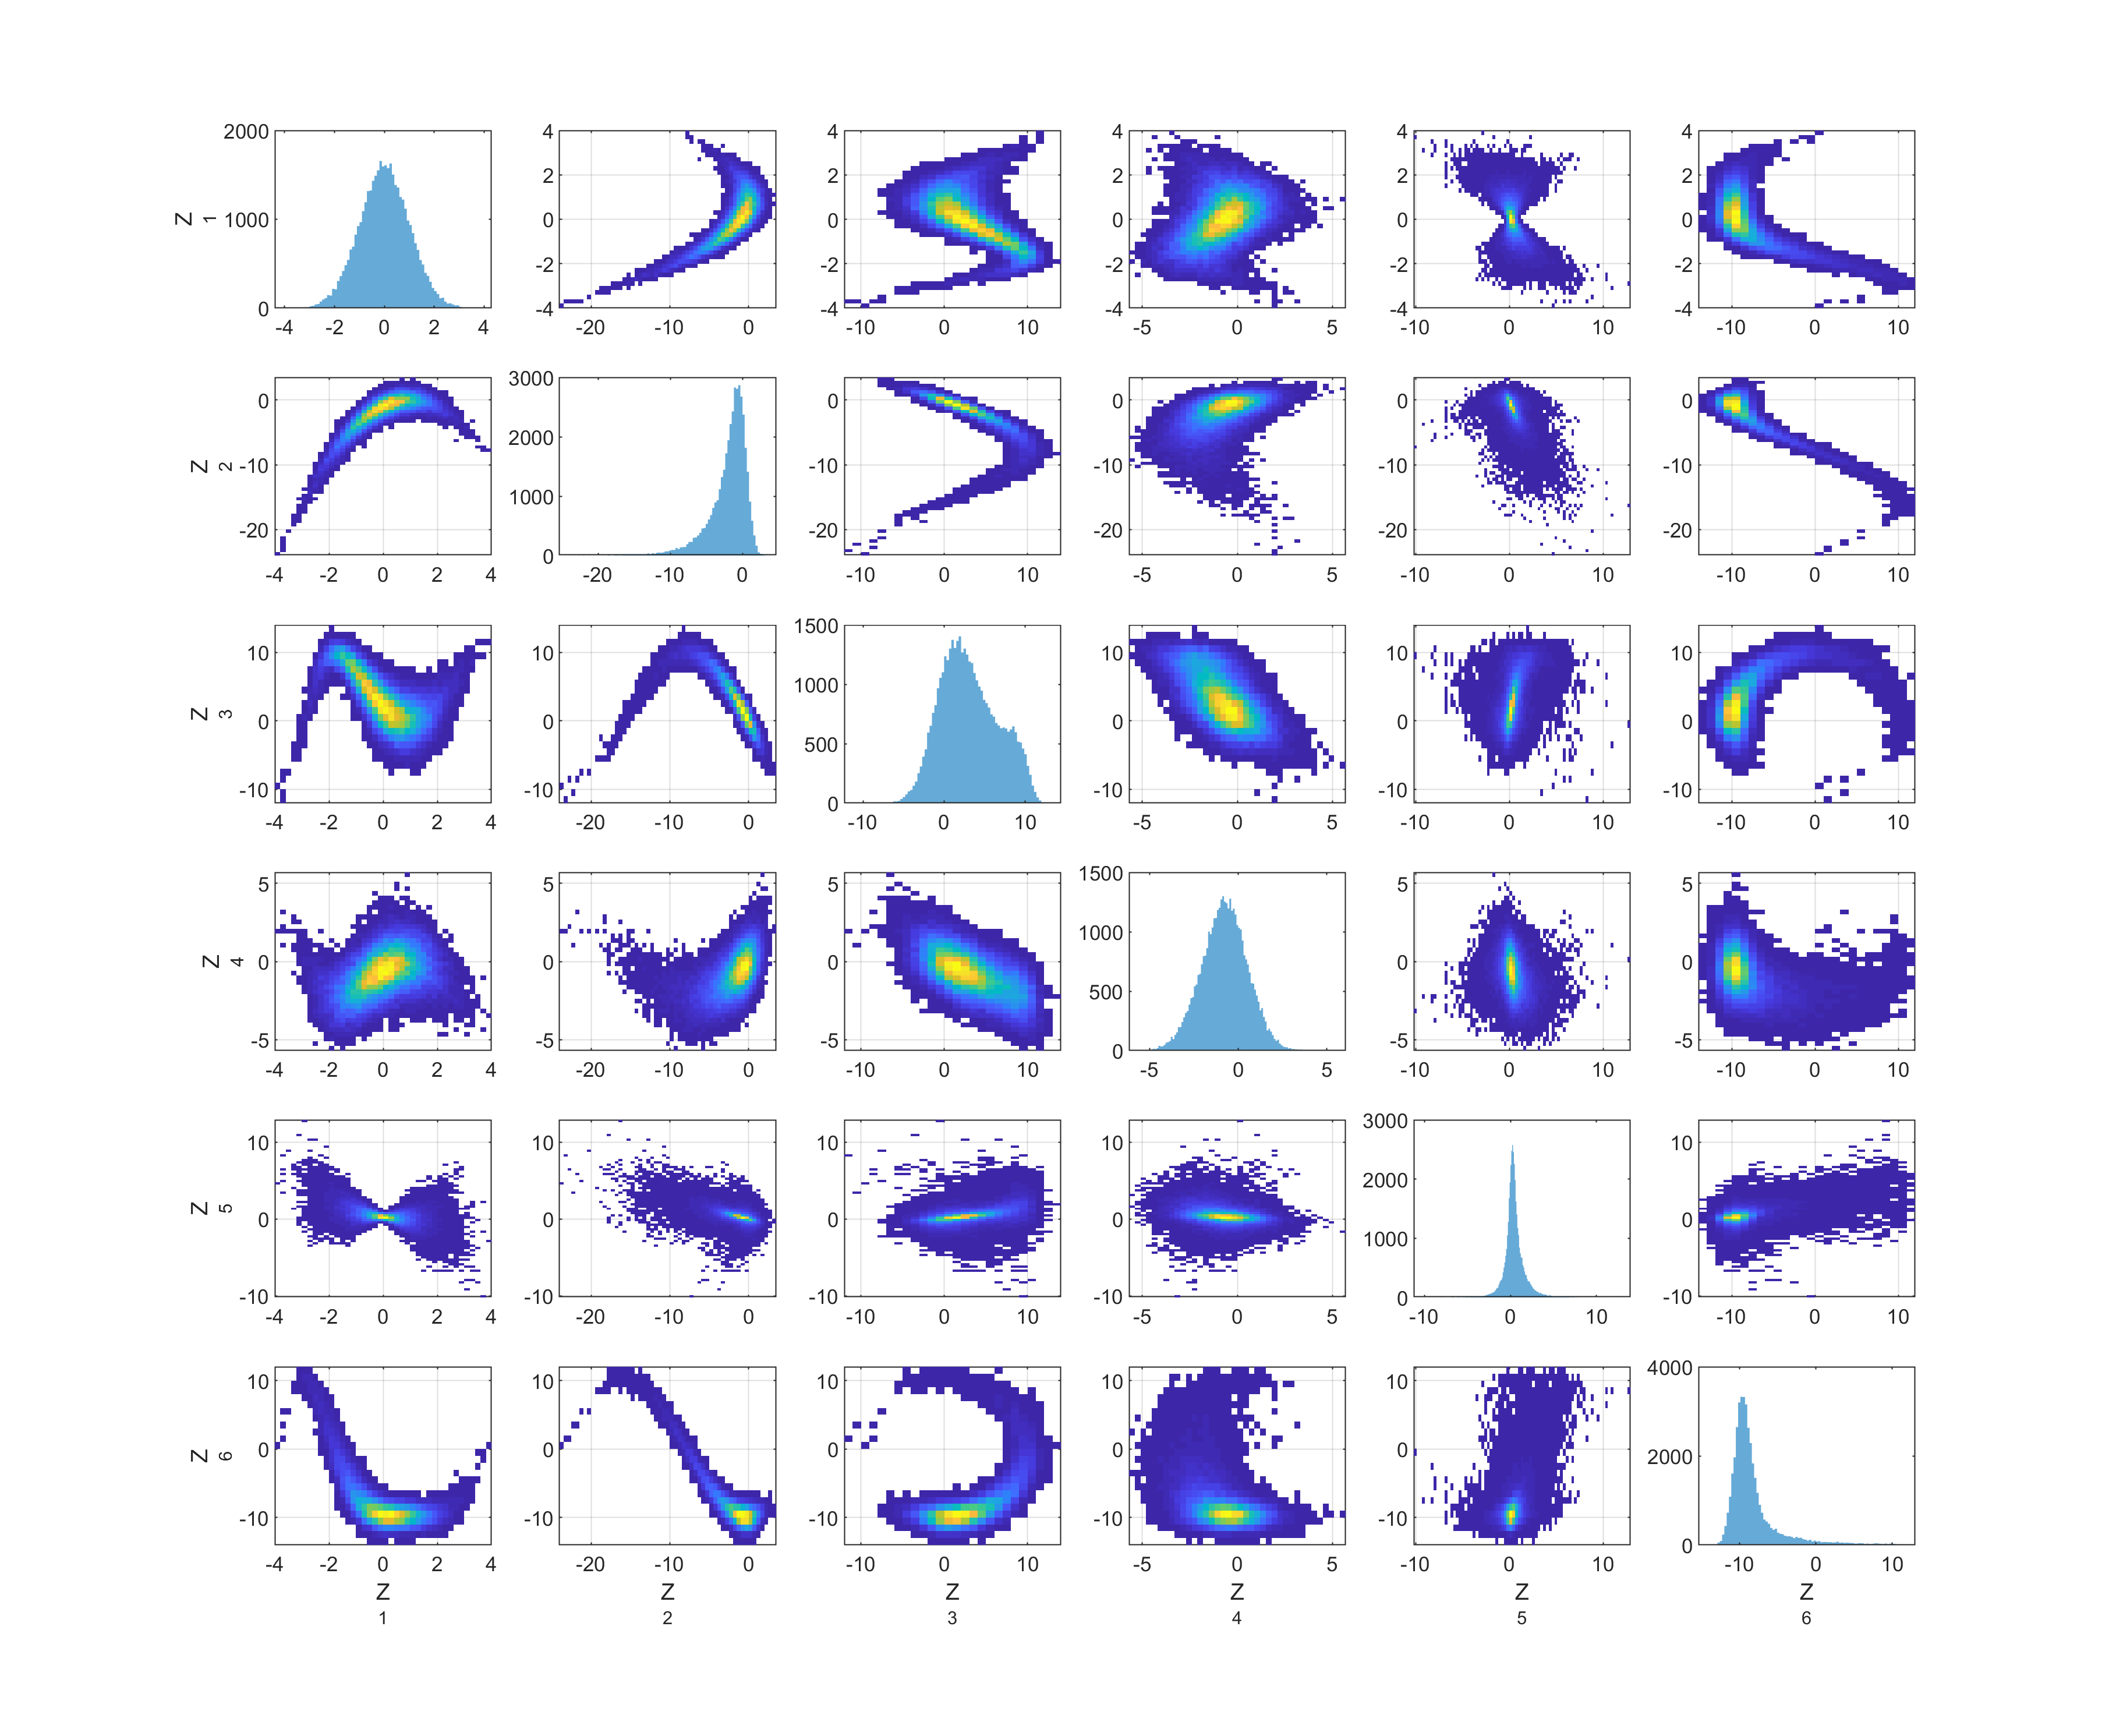
\includegraphics[width=0.75\textwidth]{figs_rev1/uncond_distribution_reference.png}
\caption{ Caption here. Image from \cite{de2021direct}.}
\label{fig:Figure1}
\end{figure}

This section includes an example of table (Table \ref{tab:Table1}).

\begin{table}
\centering
\caption{Example of table.}
\label{tab:Table1}
\begin{tabular}{ |c||c|c|c|} 
 \hline
     & $a$  &  $b$  &  $c$\\ 
 \hline 
 \hline
$a$ & 0.014 &  0.20    &   0.13  \\
\hline
$b$ & 0.20    &   0.17    &   2.46    \\
\hline
$c$ & 0.13    &   2.5     &   0.31   \\
\hline
\end{tabular} 
\end{table}


\subsection{Subsection}

Text ...

\section{Conclusions}

Conclusions here...

\section{Acknowledgments}

The authors would like to acknowledge ...

\newpage

\textbf{Code availability section}

Name of the code/library

Contact: e-mail and phone number

Hardware requirements: ...

Program language: ...
 
Software required: ...

Program size: ...

The source codes are available for downloading at the link:
https://github.com/ . . . . 


\bibliographystyle{cas-model2-names}
\bibliography{bibliography} 

\end{document}

